\section{Equations and parameters of the benchmark systems}\label{app:systems}

\textbf{Chua circuit}~\cite{Leonov2011PLA,GuanXie2025}:
\begin{equation*}
\begin{split}
&\dot x=\alpha\bigl(y-x-f(x)\bigr),\quad \dot y=x-y+z,\\
&\dot z=-(\beta y+\gamma z),\\
&f(x)=m_1x+\tfrac12(m_0-m_1)\bigl(|x+1|-|x-1|\bigr).
\end{split}
\end{equation*}
The parameters $(\alpha,\beta,\gamma,m_0,m_1)$ are
\begin{equation*}
\begin{split}
&\text{set I: } (8.4562,\ 12.0732,\ 0.0052,\ -0.1768,\ -1.1468),\\
&\text{set II: } (8.4,\ 12,\ -0.005,\ -1.2,\ -0.05).
\end{split}
\end{equation*}
For set II, the known regimes are the cycle LC, which passes through $(-7.287,\allowbreak -2.773,\allowbreak 36.02)$, and the chaotic attractors, which pass through $(1.528,\allowbreak 0.283,\allowbreak -1.819)$ and $(-1.304,\allowbreak 0.029,\allowbreak 2.387)$. The two coupled circuits of section~\ref{sec:coupled} obey
\begin{equation*}
\dot x_u=\alpha(y_u-x_u-f(x_u))+\epsilon(\bar x-x_u),\qquad \bar x=(x_1+x_2)/2,
\end{equation*}
with the other equations unchanged, in the region $B^2$.

The hidden attractors of level A are shown in Figure~\ref{fig:gallery3d}, and the five coexisting attractors of the Chua circuit with parameter set~II, together with their basins in a plane section, in Figure~\ref{fig:chuaII}.

\begin{figure}[tbhp]
\centering
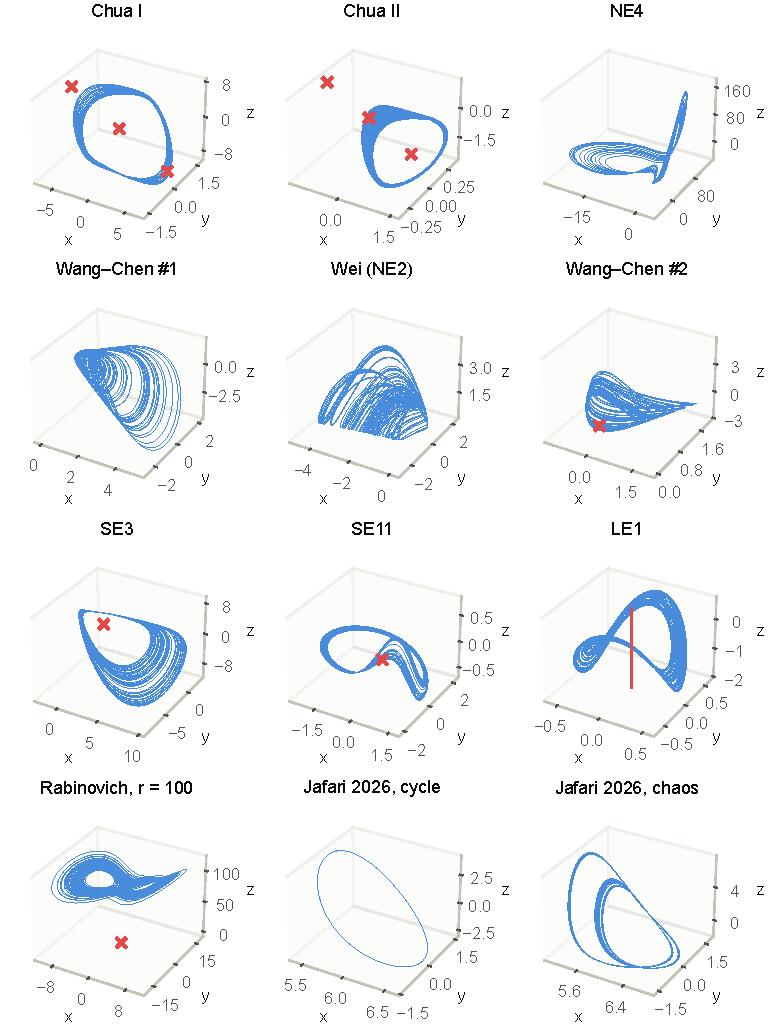
\includegraphics[width=\textwidth]{figures/fig32_gallery_3d.pdf}
\caption{Hidden attractors of the level-A benchmark. Crosses mark equilibria; for LE1, the red line is the line of equilibria $x=y=0$. NE4, Wang--Chen \#1, Wei, and the Jafari 2026 system have no equilibria, and in Wang--Chen \#2, SE3, and SE11, the single equilibrium is stable, so all attractors shown are hidden by definition.}
\label{fig:gallery3d}
\end{figure}

\begin{figure}[tbhp]
\centering
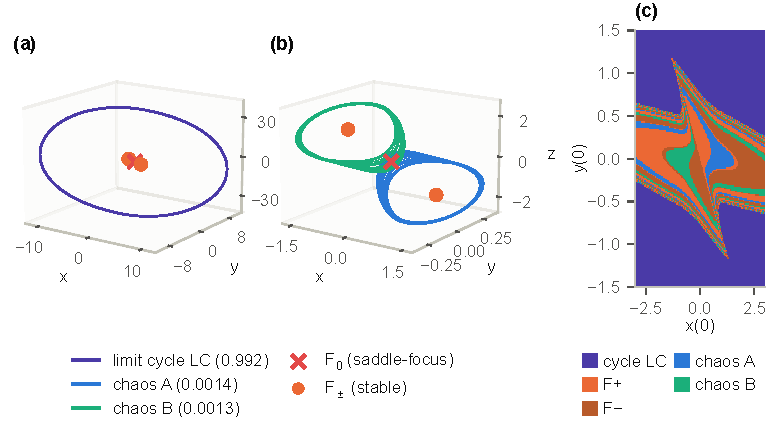
\includegraphics[width=\textwidth]{figures/fig31_chua_II_coexisting.pdf}
\caption{Chua circuit, parameter set II: five coexisting attractors. (a) The large limit cycle LC (basin fraction in the box 0.992), the chaotic attractors A and B (0.0014 and 0.0013), the saddle-focus F$_0$, and the stable foci F$_\pm$. (b) Enlarged view; the chaotic attractors surround F$_\pm$. (c) Basins in the plane $z(0)=0$ (window $|x|\le3$, $|y|\le1.5$, axes not to scale). The basins of the chaotic attractors are narrow strips between the basins of F$_\pm$ and of the cycle; a search can exploit only these boundaries and the long transients near them.}
\label{fig:chuaII}
\end{figure}


\textbf{Systems without equilibria.} NE4: $\dot x=-0.1y+a$, $\dot y=x+z$, $\dot z=xz-3y$, $a=1$. Wang--Chen \#1~\cite{WangChen2012}: $\dot x=y$, $\dot y=z$, $\dot z=-y+3y^2-x^2-xz+a$, $a=-0.05$. Wei~\cite{Wei2011}: $\dot x=-y$, $\dot y=cx+z$, $\dot z=ay^2+xz-d$, $(a,c,d)=(2,1,0.35)$. Jafari et al.\ 2026~\cite{Jafari2026NoPP}: $\dot x=y$, $\dot y=z$, $\dot z=a_1z+a_2xy+a_3yz+a_4zx+a_5$, $(a_1,a_2,a_4,a_5)=(6,-1,-1,-1)$; there is a cycle at $a_3=-1$ and chaos at $a_3=-3.548$, with the state $(6.7445,0.4214,-1.7846)$ on the attractor.

\textbf{Systems with a single stable equilibrium.} Wang--Chen \#2~\cite{WangChen2012}: $\dot x=yz+a$, $\dot y=x^2-y$, $\dot z=1-4x$, $a=0.006$. SE3~\cite{Molaie2013}: $\dot x=y$, $\dot y=z$, $\dot z=-3.4x-y-4z+y^2+xy$. SE11~\cite{Molaie2013}: $\dot x=y$, $\dot y=-x+yz$, $\dot z=-y-12z+x^2+9xz-1$.

\textbf{A system with a line of equilibria.} LE1~\cite{JafariSprott2013}: $\dot x=y$, $\dot y=-x+yz$, $\dot z=-x-axy-bxz$, $(a,b)=(15,1)$; the equilibria $(0,0,z)$ are stable for $z<0$.

\textbf{Rabinovich system}~\cite{Kuznetsov2018Rabinovich}: $\dot x=-\sigma(x-y)-ayz$, $\dot y=rx-y-xz$, $\dot z=-bz+xy$, $\sigma=-ar$; $(r,a,b)=(100,-0.009965,0.077454)$ (hidden attractor) and $(6.8,-0.5,0.99)$ (transient set~\cite{SprottMunmuangsaen2018Comment}).

\textbf{Negative control.} The Lorenz system $\dot x=a(y-x)$, $\dot y=rx-y-xz$, $\dot z=xy-bz$ at $(a,r,b)=(4,29,2)$.

\textbf{Maps.} Huynh et al.~\cite{Huynh2019}: $x'=x+y$, $y'=y-a|y|-xy+bx^2-cy^2+d$, $(a,b,c,d)=(0.01,0.1,2,0.1)$. The general family of Jiang et al.~\cite{Jiang2016Maps}: $x'=y$, $y'=a_1x+a_2y+a_3x^2+a_4y^2+a_5xy+a_6$; the cases used and their coefficients $(a_1,\dots,a_6)$ are listed below.
\begin{itemize}
\item NF I e: $(1,0,0,-0.3,0.3,2.98)$, box $[-8,8]^2$.
\item NF I f: $(1,0,0,0.38,-0.38,-1.6)$, box $[-5,5]^2$.
\item NF I g: $(1,0,0,0.12,-0.12,-3.62)$, box $[-8,8]^2$.
\item NF I i: $(1,0,0,-0.3,0.3,1.09)$, box $[-5,5]^2$.
\item SF I a: $(-0.33,0.17,-0.48,0.47,0.01,-0.9)$, box $[-5,5]^2$.
\item SF I b: $(-0.84,0,0,0.15,-0.15,-5.85)$, box $[-12,12]^2$.
\item SF I c: $(-0.99,0,0,0.23,-0.23,-4.24)$, box $[-10,10]^2$.
\item SF I d: $(-1.29,2,-0.35,-0.85,1.2,0.17)$, box $[-5,5]^2$.
\end{itemize}
The same family in the form of Ref.~\cite{Ouannas2018}: $x'=y$, $y'=x+a_1x^2+a_2y^2-a_3xy-a_4$, with the parameter sets $(0.2,0.71,0.91,1.14)$, $(0.51,1,1.51,0.74)$, and $(0.6,1,1.6,0.72)$ (``Jiang--Ouannas 1--3'' in Table~\ref{tab:integration}).

\textbf{Four-dimensional systems.} Li and Sprott~\cite{LiSprott2014}: $\dot x=y-x$, $\dot y=-xz+u$, $\dot z=xy-a$, $\dot u=-by$ at $(a,b)=(6,0.1)$, $(7,0.1)$, and $(2.6,0.44)$. Jahanshahi et al.~\cite{Jahanshahi2019}: $\dot x=y$, $\dot y=z$, $\dot z=w$, $\dot w=-aw+bx^2-cy^2+exy+fxz+g$, $(a,b,c,e,f,g)=(1.05,0.7,0.19,1.37,1.79,1.15)$.

\textbf{Synthetic families} D1 and D2 are given by \eqref{eq:d1} and \eqref{eq:d2} with SE3 as the base system, in the region $B=[-10,10]^3\times[-1,1]^m$, $m=1$--11, and are integrated with the settings of SE3; in D2, the transient segment is extended by $\ln(\sqrt m/\rho)/\kappa+5$ time units so that every escaping trajectory leaves before the observation window starts.

The integration parameters and the regions of initial conditions are listed in Table~\ref{tab:integration}, including those of the control systems. Figure~\ref{fig:chuaI} shows the Chua circuit with parameter set I, Figure~\ref{fig:jafari} the chaos window of the Jafari 2026 system, Figure~\ref{fig:maps} the level-B maps, and Figure~\ref{fig:levelA} the level-C system of Li and Sprott.

\begin{table}[tbhp]
\centering
\caption{Integration parameters and regions of initial conditions $B$. For flows, the lengths of the transient segment and of the observation window are given in time units; for maps, in iterations. $R_{\rm esc}$ is the escape radius.}
\label{tab:integration}

\resizebox{\textwidth}{!}{%
\begin{tabular}{lrlrlr}
\toprule
System & $n$ & Integration & $T_{\rm tr}/T_{\rm obs}$ & Region $B$ & $R_{\rm esc}$ \\
\midrule
Chua I & 3 & RK4, $\Delta t=0.0025$ & 1000 / 100 & $[-10,10]^2\times[-15,15]$ & 100 \\
Chua II & 3 & RK4, $\Delta t=0.0025$ & 1000 / 100 & $[-10,10]^2\times[-15,15]$ & 100 \\
NE4 & 3 & RK4, $\Delta t=0.001$ & 500 / 500 & $[-40,20]\times[-30,50]\times[-80,220]$ & 2000 \\
Wang--Chen \#1 & 3 & RK4, $\Delta t=0.01$ & 300 / 100 & $[-10,10]^3$ & 100 \\
Wei (NE2) & 3 & RK4, $\Delta t=0.01$ & 300 / 100 & $[-10,10]^3$ & 100 \\
Jafari 2026, $a_3=-1$ & 3 & RK4, $\Delta t=0.01$ & 3000 / 200 & $[-10,10]^3$ & 60 \\
Jafari 2026, $a_3=-3.548$ & 3 & RK4, $\Delta t=0.005$ & 1000 / 200 & $[-10,10]^3$ & 60 \\
Wang--Chen \#2 & 3 & RK4, $\Delta t=0.01$ & 300 / 100 & $[-10,10]^3$ & 100 \\
SE3 & 3 & RK4, $\Delta t=0.01$ & 300 / 100 & $[-10,10]^3$ & 100 \\
SE11 & 3 & RK4, $\Delta t=0.01$ & 300 / 100 & $[-10,10]^3$ & 100 \\
LE1 & 3 & RK4, $\Delta t=0.01$ & 300 / 100 & $[-10,10]^3$ & 100 \\
Rabinovich, $r=100$ & 3 & RK4, $\Delta t=0.002$ & 200 / 100 & $[-60,60]^2\times[-150,150]$ & 1000 \\
Rabinovich, $r=6.8$ & 3 & RK4, $\Delta t=0.005$ & 300 / 100 & $[-10,10]^2\times[-10,15]$ & 200 \\
Lorenz $(4,29,2)$ & 3 & RK4, $\Delta t=0.005$ & 300 / 100 & $[-20,20]^2\times[0,50]$ & 500 \\
D1, D2 (base SE3) & $3+m$ & RK4, $\Delta t=0.01$ & $\ge300$ / 100 & $[-10,10]^3\times[-1,1]^m$ & 100 \\
Huynh 2019 & 2 & iterations & 20\,000 / 5000 & $[-3,3]^2$ & 100 \\
Jiang NF I e & 2 & iterations & 20\,000 / 5000 & $[-8,8]^2$ & 1000 \\
Jiang NF I f & 2 & iterations & 20\,000 / 5000 & $[-5,5]^2$ & 1000 \\
Jiang NF I g & 2 & iterations & 20\,000 / 5000 & $[-8,8]^2$ & 1000 \\
Jiang NF I i & 2 & iterations & 20\,000 / 5000 & $[-5,5]^2$ & 1000 \\
Jiang SF I a & 2 & iterations & 20\,000 / 5000 & $[-5,5]^2$ & 1000 \\
Jiang SF I b & 2 & iterations & 20\,000 / 5000 & $[-12,12]^2$ & 1000 \\
Jiang SF I c & 2 & iterations & 20\,000 / 5000 & $[-10,10]^2$ & 1000 \\
Jiang SF I d & 2 & iterations & 20\,000 / 5000 & $[-5,5]^2$ & 1000 \\
Jiang--Ouannas 1--3 & 2 & iterations & 20\,000 / 5000 & $[-2,2]^2$ & 100 \\
H\'enon (control) & 2 & iterations & 5000 / 2000 & $[-2,2]^2$ & 50 \\
Li--Sprott 4D, $a=6$ & 4 & RK4, $\Delta t=0.005$ & 500 / 200 & $[-15,15]^4$ & 500 \\
Li--Sprott 4D, $a=7$ & 4 & RK4, $\Delta t=0.005$ & 500 / 200 & $[-15,15]^4$ & 500 \\
Li--Sprott 4D, hyperchaos & 4 & RK4, $\Delta t=0.005$ & 500 / 200 & $[-15,15]^4$ & 500 \\
Jahanshahi 4D & 4 & RK4, $\Delta t=0.005$ & 500 / 200 & $[-10,10]^4$ & 500 \\
Coupled Chua II, $\epsilon=0.1$ & 6 & RK4, $\Delta t=0.0025$ & 1000 / 100 & $\bigl([-10,10]^2\times[-15,15]\bigr)^2$ & 141 \\
\bottomrule
\end{tabular}%
}

\end{table}

\begin{figure}[tbhp]
\centering
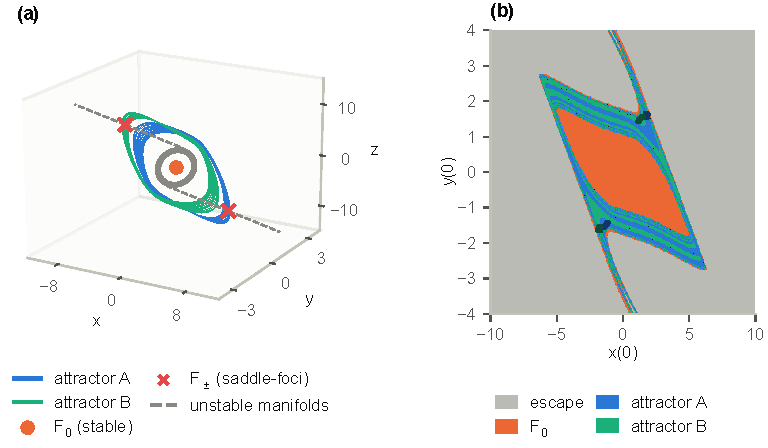
\includegraphics[width=\textwidth]{figures/fig30_chua_I_hidden.pdf}
\caption{Chua circuit, parameter set I. (a) Two symmetric hidden chaotic attractors A and B, the stable focus-node F$_0$ (dot), the saddle-foci F$_\pm$ (crosses), and their unstable manifolds. One branch of each manifold escapes to infinity and the other winds onto F$_0$, so the standard procedure does not find attractors A and B. (b) Basins in the plane $z(0)=0$ (window $|y|\le4$). Gray: escape to infinity; orange: F$_0$; blue and green: attractors A and B; dark points: the attractors in the layer $|z|<0.15$.}
\label{fig:chuaI}
\end{figure}

\begin{figure}[tbhp]
\centering
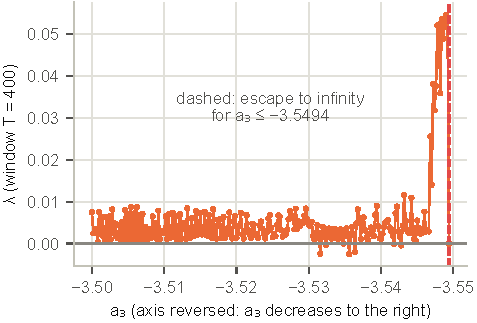
\includegraphics[width=0.62\textwidth]{figures/fig35_jafari2026.pdf}
\caption{System of Jafari et al.~\cite{Jafari2026NoPP} without fixed or perpetual points: the Lyapunov exponent over windows of length $T=400$ in the narrow chaos window near the boundedness limit ($a_3$ decreases to the right); for $a_3\le-3.5494$, trajectories escape to infinity. The cycle at $a_3=-1$ and the chaotic attractor at $a_3=-3.548$ are shown in Figure~\ref{fig:gallery3d}.}
\label{fig:jafari}
\end{figure}

\begin{figure}[tbhp]
\centering
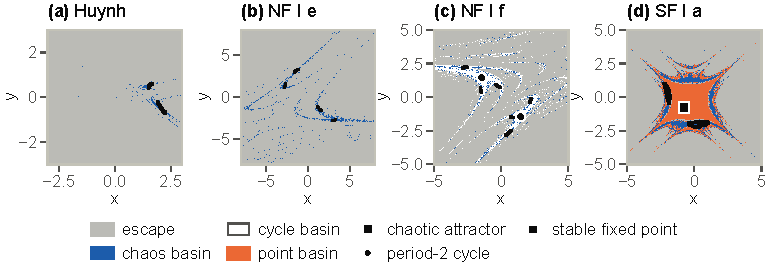
\includegraphics[width=\textwidth]{figures/fig34_maps_phase_basin.pdf}
\caption{Two-dimensional maps of level B: phase--basin portraits. (a) The map of Huynh et al.~\cite{Huynh2019} without fixed points ($p=0.0091$ in $[-3,3]^2$). (b), (c) Cases NF~I~e and NF~I~f of the family of Jiang et al.~\cite{Jiang2016Maps} without fixed points; in NF~I~f, a chaotic attractor coexists with a period-2 cycle (markers). (d) Case SF~I~a with a single stable fixed point (square). Light gray: escape; dark blue: basin of the chaotic attractor; white: basin of the cycle; orange: basin of the fixed point; black: the attractor.}
\label{fig:maps}
\end{figure}

\begin{figure}[tbhp]
\centering
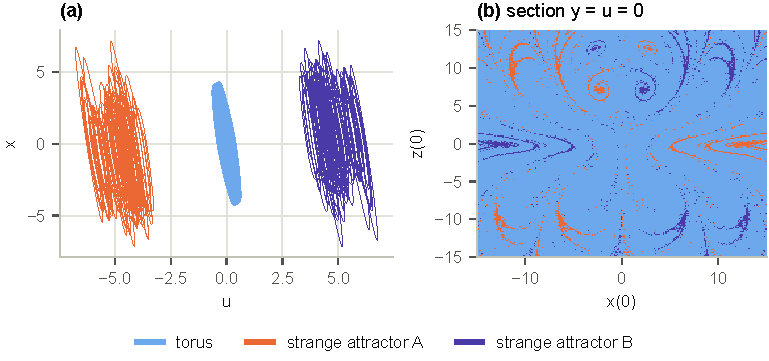
\includegraphics[width=\textwidth]{figures/fig33_li_sprott_4d.pdf}
\caption{Four-dimensional simplified Lorenz system~\cite{LiSprott2014} at $a=6$, $b=0.1$, which has no equilibria. (a) The torus (basin fraction 0.090) and a pair of symmetric strange attractors ($\lambda\approx0.25$; 0.446 and 0.464) in the projection $(u,x)$. (b) Basins in the section $y=u=0$ of the box $[-15,15]^4$; the torus occupies the ``background,'' and the strange attractors form spiral tongues. Here the rare target is the torus, not the chaos.}
\label{fig:levelA}
\end{figure}

